\chapter{Scalability Experiments}
\label{ch:scalability}

The assignment brief singles out scalability as the experiment to look at
in particular, and it is also the property the paper's central claim rests
on but never measures in a distributed setting: every timing number in
the paper's own Table~3 comes from a single-threaded Java process. This
chapter measures training time per iteration along the three axes that
matter for a Spark deployment: the number of latent factors $K$ (Section
\ref{sec:scale_k}), the degree of parallelism (Section~\ref{sec:scale_par}),
and the size of the training set (Section~\ref{sec:scale_data}), and closes
with a comparison against Spark MLlib's own implicit-feedback ALS
(Section~\ref{sec:scale_mllib}). Every run in this chapter uses $c_0=512$,
$\alpha=0.4$ (the values selected in Section~\ref{sec:weighting}) and
$\lambda=0.01$, and reports wall-clock time averaged over 3 iterations to
smooth out one-off scheduling noise. Three iterations is enough to
measure timing reliably but not enough to reach the converged accuracy of
Chapter~\ref{ch:results}, so the HR@10/NDCG@10 values reported alongside the
timings in this chapter should be read only as a sanity check that the
model is learning something reasonable, not as final accuracy numbers.
The configuration $K=32$, full training set, 8 partitions is the shared
baseline across all three sweeps below, so it gets measured three times
independently: 11.54\,s (Section~\ref{sec:scale_k}), 10.41\,s
(Section~\ref{sec:scale_par}), and 10.76\,s (Section~\ref{sec:scale_data}).
The roughly 10\% spread between these three nominally identical runs is a
useful, honest indicator of the run-to-run timing noise on this machine (a
single Spark session, no isolation from background load), and it sets a
rough lower bound on how precisely any single number in this chapter
should be trusted.

\section{Scaling with the number of latent factors}
\label{sec:scale_k}

\begin{figure}[H]
\centering
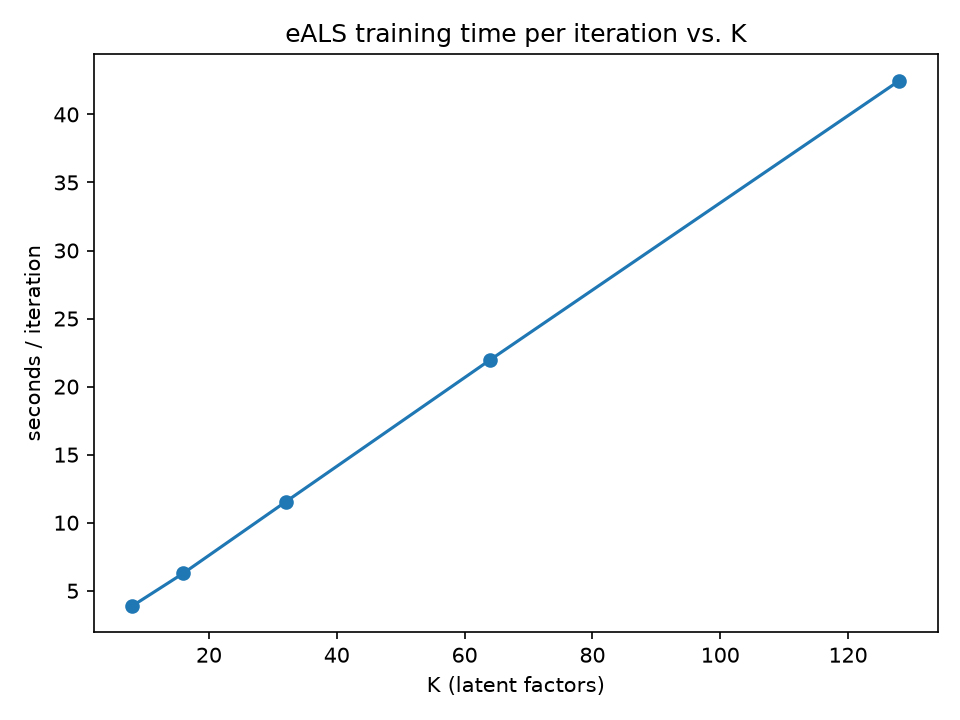
\includegraphics[width=0.65\textwidth]{figures/scalability_K.png}
\caption{eALS training time per iteration versus $K$, on the full training
set (925{,}660 interactions), 8 partitions.}
\label{fig:scale_k}
\end{figure}

Table~\ref{tab:scale_k} lists the raw numbers behind Figure~\ref{fig:scale_k}.
Going from $K=8$ to $K=128$, a $16\times$ increase, training time per
iteration grows from 3.88\,s to 42.47\,s, a $10.9\times$ increase. This is
the single most direct confirmation of the paper's central efficiency
claim available from this project: a classical vector-wise ALS solver with
genuine $O(K^3)$ matrix inversion would need roughly $16^3 = 4096\times$
more time for the same change in $K$, whereas eALS's element-wise updates
grow \emph{sub-linearly relative to that cubic bound}, and not far off
linear in absolute terms.

\begin{table}[H]
\centering
\begin{tabular}{rrrr}
\toprule
$K$ & seconds/iteration & HR@10 (3 iters) & NDCG@10 (3 iters) \\
\midrule
8   & 3.88  & 0.471 & 0.293 \\
16  & 6.29  & 0.530 & 0.337 \\
32  & 11.54 & 0.569 & 0.373 \\
64  & 21.97 & 0.561 & 0.375 \\
128 & 42.47 & 0.547 & 0.370 \\
\bottomrule
\end{tabular}
\caption{Training time and (under-trained, 3-iteration) accuracy versus
$K$.}
\label{tab:scale_k}
\end{table}

It helps to be precise about why growth is close to linear rather than
exactly linear, since the theoretical complexity
$O((M+N)K^2+|\mathcal{R}|K)$ from Section~\ref{sec:ealsdesign} has both a
quadratic and a linear term in $K$. At this dataset's scale
($M+N\approx55{,}227$, $|\mathcal{R}|\approx925{,}660$), the $O((M+N)K^2)$
term, dominated by the $S^q=\sum_i c_i q_i q_i^\top$ and $S^p=P^\top P$
matrix products computed once per sweep via NumPy's BLAS-backed matrix
multiplication, and the $O(|\mathcal{R}|K)$ term, the per-user,
per-item Python loop of Listing~\ref{lst:update_users}, are of comparable
magnitude and grow at different rates, so the observed curve is a mix of
both rather than a pure power law in $K$. The accuracy figures in the same
table should not be read as ``larger $K$ hurts'': they are measured after
only 3 iterations, and larger $K$ needs more iterations to reach the same
degree of convergence as smaller $K$, not fewer.

\section{Scaling with parallelism}
\label{sec:scale_par}

\begin{figure}[H]
\centering
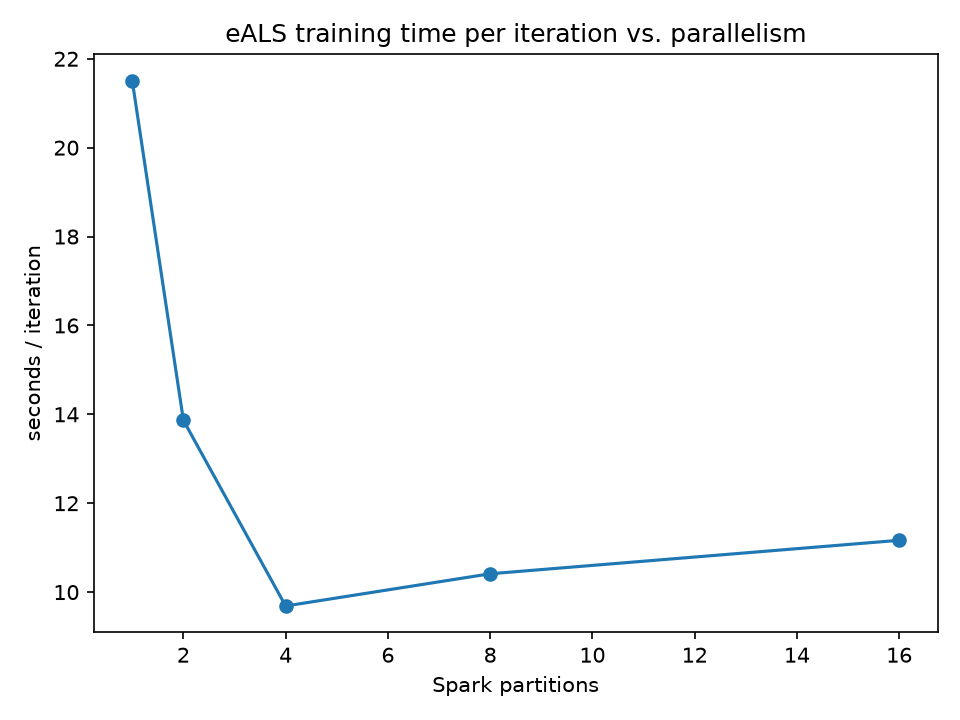
\includegraphics[width=0.65\textwidth]{figures/scalability_partitions.png}
\caption{eALS training time per iteration versus the number of Spark
partitions, $K=32$, full training set.}
\label{fig:scale_par}
\end{figure}

Table~\ref{tab:scale_par} shows time per iteration as the user/item id
space is split across 1, 2, 4, 8, and 16 partitions, on a single machine
running Spark in local mode.

\begin{table}[H]
\centering
\begin{tabular}{rr}
\toprule
partitions & seconds/iteration \\
\midrule
1  & 21.50 \\
2  & 13.87 \\
4  & 9.69 \\
8  & 10.41 \\
16 & 11.17 \\
\bottomrule
\end{tabular}
\caption{Training time per iteration versus Spark partition count.}
\label{tab:scale_par}
\end{table}

Going from 1 to 4 partitions roughly halves-then-halves-again the time per
iteration (21.5\,s down to 9.7\,s), confirming that the update really is
being distributed and not just serialized through Spark's job machinery for
no benefit. Beyond 4 partitions, though, time per iteration \emph{increases}
slightly rather than continuing to fall: 10.4\,s at 8 partitions,
11.2\,s at 16. This is not a flaw in the parallelization strategy described
in Section~\ref{sec:parallel}; it is what happens when the fixed
per-partition overhead (task scheduling, serializing the broadcast
variables' handles, collecting results back to the driver) stops being
negligible relative to the shrinking amount of actual work each partition
does. With only 4 CPU cores available on the machine these experiments ran
on, splitting the work into 16 partitions means each one gets roughly a
quarter of a core's worth of genuine work between two and four times a
second, which is exactly the regime where Spark's per-task overhead starts
to dominate. Section~\ref{sec:weaknesses} discusses what this does and does
not say about behaviour on an actual multi-node cluster, which is the
setting the paper's parallelism argument is really aimed at.

\section{Scaling with training-set size}
\label{sec:scale_data}

\begin{figure}[H]
\centering
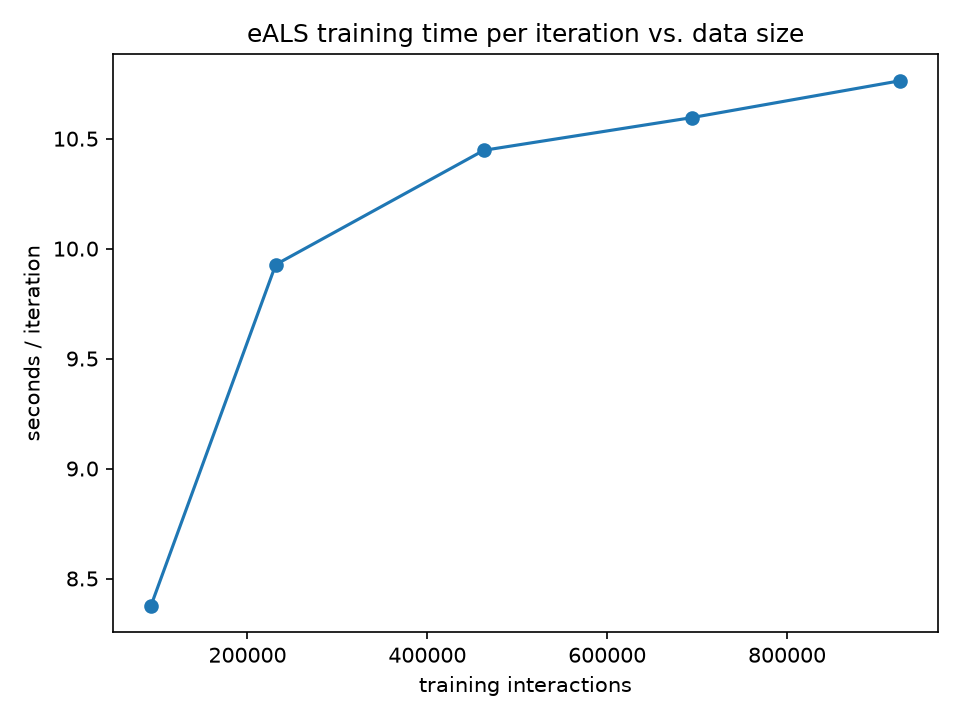
\includegraphics[width=0.65\textwidth]{figures/scalability_data_size.png}
\caption{eALS training time per iteration versus training-set size ($K=32$,
8 partitions), from 10\% to 100\% of the 925{,}660 training interactions.}
\label{fig:scale_data}
\end{figure}

Table~\ref{tab:scale_data} is the most surprising result in this chapter.
Increasing the training set tenfold, from 92{,}566 to 925{,}660
interactions, increases time per iteration by only $1.29\times$ (8.38\,s to
10.76\,s). That is almost flat, where the $O(|\mathcal{R}|K)$ term of the
complexity analysis would predict something much closer to linear ($10\times$).

\begin{table}[H]
\centering
\begin{tabular}{rrr}
\toprule
fraction of training data & interactions & seconds/iteration \\
\midrule
0.10 & 92{,}566  & 8.38 \\
0.25 & 231{,}415 & 9.93 \\
0.50 & 462{,}830 & 10.45 \\
0.75 & 694{,}245 & 10.60 \\
1.00 & 925{,}660 & 10.76 \\
\bottomrule
\end{tabular}
\caption{Training time per iteration versus training-set size, $M$ and $N$
held fixed.}
\label{tab:scale_data}
\end{table}

The explanation is the same fixed-versus-variable-cost split noted in
Section~\ref{sec:scale_k}: subsampling the training \emph{interactions}
does not shrink $M$ or $N$ (a user or item can lose most of its
interactions and still exist in the model), so the $O((M+N)K^2)$ term,
made up of the two matrix-cache computations plus the fixed cost of
dispatching Spark jobs over the full $M$-user and $N$-item id space
regardless of how many of them have interactions left, stays essentially
constant across
the sweep, while only the $O(|\mathcal{R}|K)$ term genuinely shrinks. At
$K=32$ on this dataset, that fixed term turns out to dominate, which is
good news for the deployment scenario the paper is actually aimed at (an
online system where the item and user catalog grows slowly but the volume
of interactions per user grows quickly): eALS's cost here is governed more
by catalog size than by interaction volume, which is the opposite of what
naive whole-data ALS complexity analysis alone would suggest without
separating the two terms in $O((M+N)K^2+|\mathcal{R}|K)$.

\section{Comparison against Spark MLlib's ALS}
\label{sec:scale_mllib}

\begin{figure}[H]
\centering
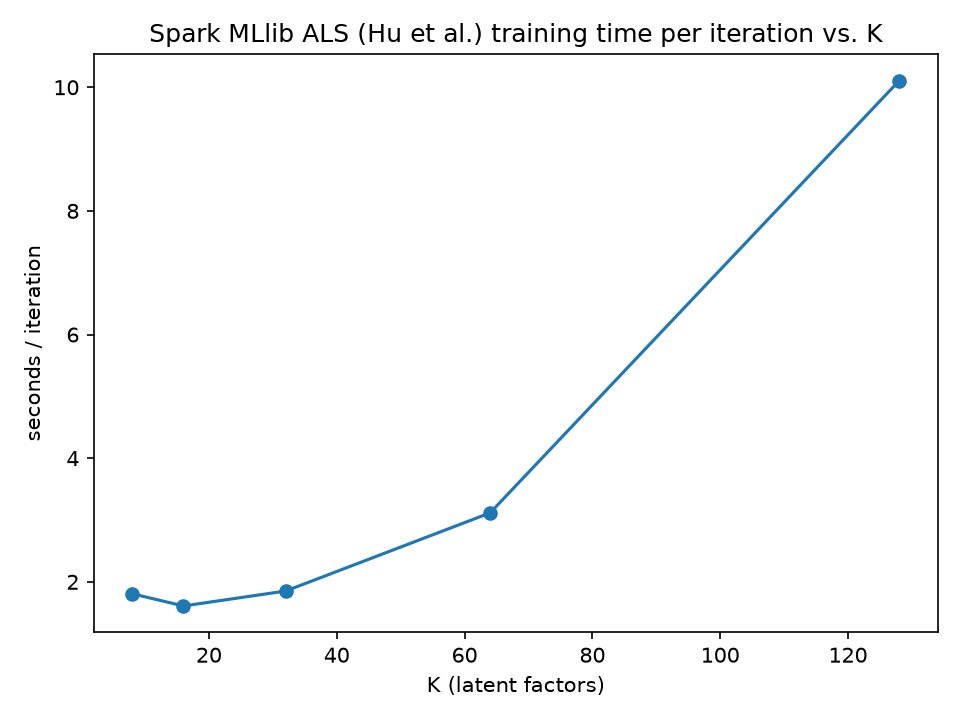
\includegraphics[width=0.65\textwidth]{figures/mllib_scalability_K.png}
\caption{Spark MLlib's \texttt{ALS(implicitPrefs=True)} training time per
iteration versus $K$, same dataset.}
\label{fig:scale_mllib}
\end{figure}

As a reference point independent of this project's own implementation,
Table~\ref{tab:scale_mllib} repeats the $K$-sweep from
Section~\ref{sec:scale_k} using Spark MLlib's built-in
\texttt{ALS(implicitPrefs=True)}, which implements Hu et al.'s uniform-weight
whole-data objective with a production-grade, JVM-native vector-wise
solver (\texttt{src/baselines.py}).

\begin{table}[H]
\centering
\begin{tabular}{rrrr}
\toprule
$K$ & seconds/iteration & HR@10 & NDCG@10 \\
\midrule
8   & 1.81  & 0.508 & 0.315 \\
16  & 1.61  & 0.545 & 0.345 \\
32  & 1.85  & 0.562 & 0.364 \\
64  & 3.12  & 0.567 & 0.374 \\
128 & 10.10 & 0.557 & 0.370 \\
\bottomrule
\end{tabular}
\caption{Spark MLlib ALS: training time and 10-iteration accuracy versus
$K$.}
\label{tab:scale_mllib}
\end{table}

MLlib's implementation is faster in absolute terms across the whole sweep.
That is unsurprising, since it is a mature, JIT-compiled Scala/Breeze
implementation running matrix inversion via a near-$O(K^{2.376})$
algorithm rather than a Python-loop-bound coordinate-descent update, and
the paper itself notes that real implementations of vector-wise ALS never
show the full $O(K^3)$ growth their asymptotic analysis predicts, for the
same reason. One entry does not fit a clean growth curve: $K=16$
(1.61\,s) is marginally faster than $K=8$ (1.81\,s), which is not
consistent with any monotonic cost model. At well under two seconds per
iteration, these runs are short enough that fixed overhead, JVM warm-up
and Spark job dispatch that does not scale with $K$ at all, plausibly
dominates whatever small, genuine $K$-dependent cost separates the two,
so this single inversion is best read as noise rather than a real
non-monotonicity in MLlib's cost. What matters for this report's argument is the \emph{shape}
of the curve, not the absolute numbers: MLlib's own timings grow
$5.6\times$ from $K=8$ to $K=128$ ($16\times$ increase in $K$), similar in
kind to eALS's $10.9\times$ growth over the same range. Both are sub-cubic,
both broadly consistent with the paper's claim that a well-implemented ALS
variant does not actually need to pay the full $O(K^3)$ its naive
complexity analysis suggests, and both a very different regime from what a
textbook matrix-inversion implementation without any of these
optimizations would show.
